\subsection{Elektronik}
Skriv om monterandet av komponenterna

\begin{figure}[H]
    \centering
    \caption{\small En av högtalarna nedmonterade}
    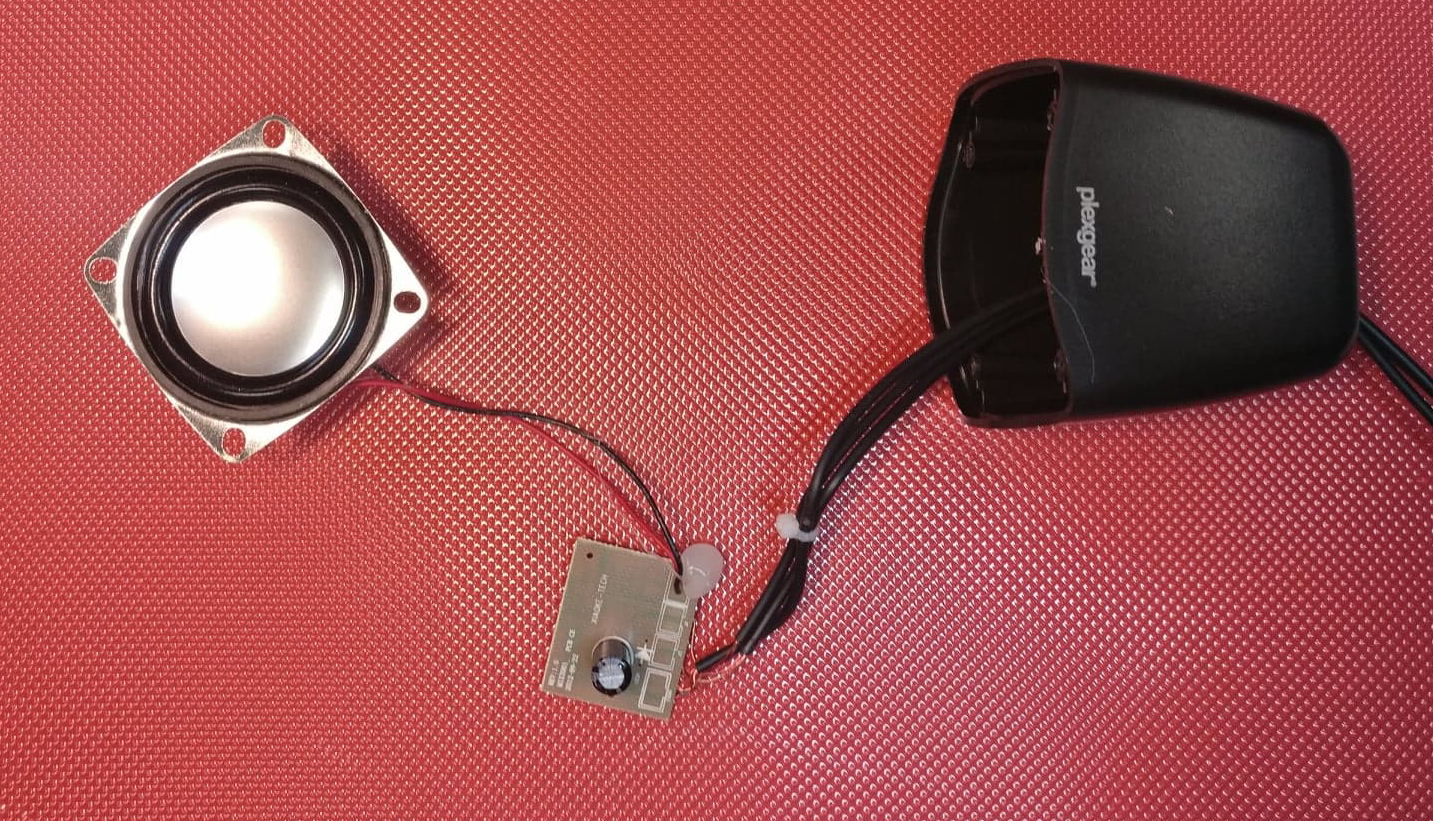
\includegraphics[width=12cm]{bilder/speaker_before_change.jpg}
\end{figure}
fiokopdfopsd
\begin{figure}[H]
    \centering
    \caption{\small Högtalarna tillsammans med den ombyggda, isolerade förstärkaren.}
    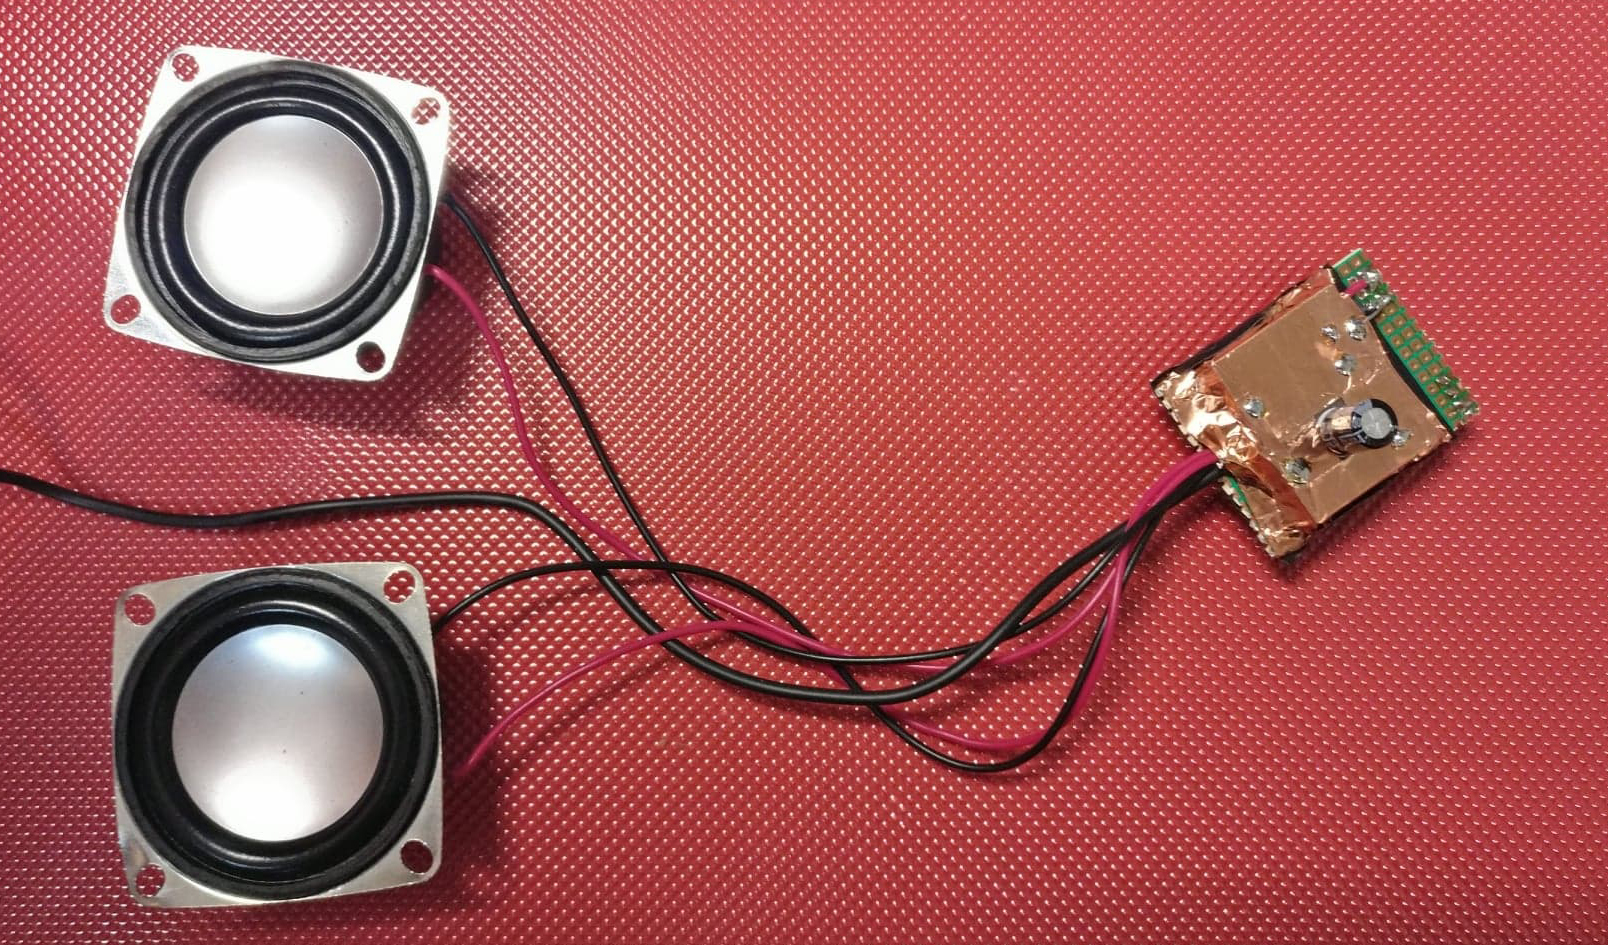
\includegraphics[width=12cm]{bilder/speakers_and_amplifier.jpg}
\end{figure}

\subsection{Mjukvara}
Som tidigare nämnt i avsnitt \ref{metod} så används mjukvaran Mycroft för att bearbeta, utföra och besvara alla kommandon och frågor som användaren ställer. 

För att enklast nyttja Mycroft-tjänsterna på en Raspberry Pi-dator så används Picroft – en fil med operativsystemet Raspbian Stretch Lite färdig\-paketerad med Mycroft \cite{picroft}. Äldre versioner av Picroft är dock inte kompatibel med Raspberry Pi modellen 3 B+.  Eftersom datormodellen i fråga är en del av detta projekt bör således den senaste versionen av Picroft (2018-9-12) användas för att mjukvaran ska fungera korrekt. För att faktiskt använda Picroft så hämtas en fil från internet och bränns sedan till ett micro-SD-kort. Minneskortet placeras i enkortsdatorn och enheten kan därefter startas.

Nästa steg i installationsprocessen är att ladda ner och installera drivrutiner till mikrofonen \cite{seeeds_documentation, reaspeker-installation}. Fabrikanten Seeeds egna drivrutiner laddas ner med hjälp av detta kommando:
\begin{minted}{bash}
git clone https://github.com/respeaker/seeed-voicecard.git
\end{minted}
Därefter installeras drivrutinerna och datorn startas om.
\begin{minted}{bash}
cd seeed-voicecard
sudo ./install.sh 4mic
sudo shutdown -r now
\end{minted}
I enkortsdatorns inbyggda konfigurationsmeny anges hålet för 3.5mm telepluggar som ljudutgång. 
\begin{minted}{bash}
sudo raspi-config
\end{minted}

För att få operativsystemet och Mycrofts röst-tjänster att korrekt använda sig av mikrofonen måste nu en asymmetrisk ljudenhet skapas i det inbyggda ljudsystemet ALSA. Detta åstadkoms genom att skapa filen \textit{~/.asoundrc} och placera följande rader kod i den:
\begin{minted}{bash}
pcm.!default {
    type asym
    playback.pcm "hw:0,0"
    capture.pcm "hw:1,0"
}
\end{minted}

Standardinställningarna som är angivna i den befintliga konfigurationsfilen \textit{/etc/asound.conf} måste även bytas ut till samma rader kod. Därefter startas datorn om. Efter omstart bör indikatorn för ljudnivå i Mycrofts användargränssnitt\footnote{Kommandot mycroft-cli-client används för att starta användargränssnittet} nu visa att mikrofonen fungerar korrekt. 
\\
SKRIV OM INTERNET-FIXEN, ändra setup wizard (eller var det någon annan fil) så att den pingar en vettig ip?
\\
Raspberry Pi-datorn har en röd lysdiod som lyser när strömmen är ansluten, detta stör rent estetiskt då det röda skenet kommer synas genom plasthöljet. Vi stänger av den genom att lägga till följande rad kod i filen \textit{/etc/rc.loca}l ovanför {\mintinline{latex}{exit 0}}: 
\begin{minted}{bash}
sudo sh -c "echo none > /sys/class/leds/led1/trigger"
\end{minted}

\subsection{Hölje och ihopmontering av enheten}
Höljet till den smarta högtalaren ritas i CAD-programmet Autodesk Inventor 2019. Höljet består av två delar, se figur \ref{fig:top-3d} och \ref{fig:bottom-3d}. I den nedre delen av högtalaren finns det skruvhål för att fästa enkortsdatorn och även hål dedikerade till ström, nätverks- och USB-ingångarna så att de alltid ska vara åtkomliga. Den övre delen av höljet har skruvhål för att fästa mikrofonkortet men även hål på sidan där högtalarna skall placeras. 
\begin{figure}[H]
    \centering
    \caption{\small Rendering av den övre halvan av höljet.}
    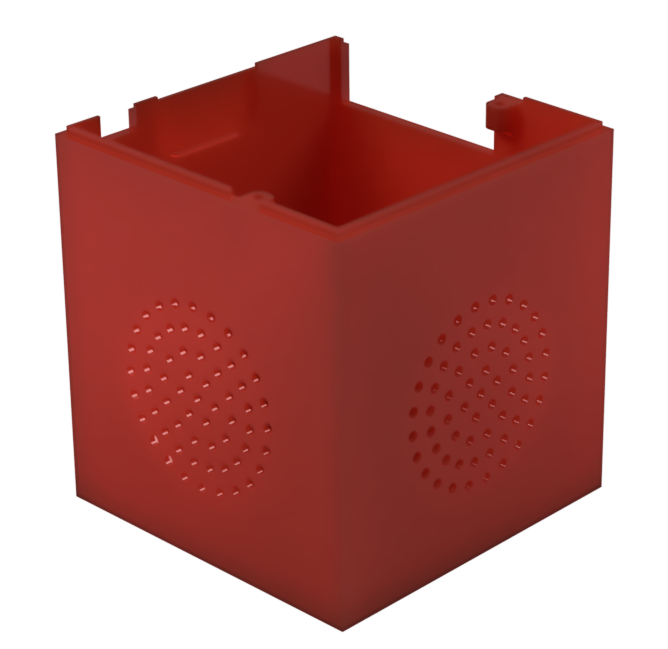
\includegraphics[width=9cm]{bilder/top_red.png}
    \label{fig:top-3d} 
\end{figure}

\begin{figure}[H]
    \centering
    \caption{\small Rendering av den nedre halvan av höljet.}
    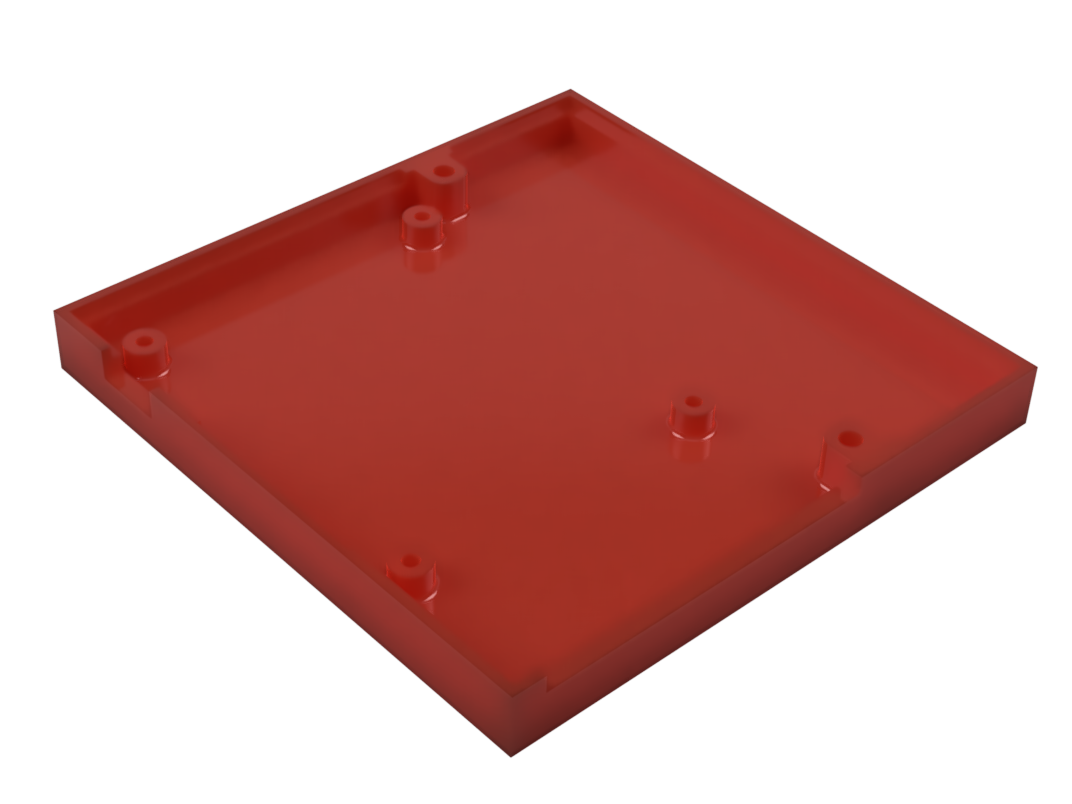
\includegraphics[width=9cm]{bilder/bottom_red.png}
    \label{fig:bottom-3d} 
\end{figure}

Efter de digitala 3D-filerna till höljet är färdigställda så produceras de två bitarna i 3D-skrivaren Ultimaker 3 med PLA-plast, i detta fallet röd sådan från skrivar\-tillverkaren själv. Det är även värt att notera att delarna är designade för att inte behövs några stödben när de skrivs ut.

När de båda delarna är utskrivna kan alla komponenter monteras i höljet. Mikrofonkortet och enkortsdatorn skruvas fast och ansluts till varandra med en flatkabel som även försörjer förstärkaren med ström. Högtalarna limmas fast på insidan, när dessa sitter fast kan slutligen höljets två delar skruvas samman och plastben klistras fast på undersidan.


\begin{figure}[H]
    \centering
    \caption{\small Bild av den färdiga prototypen.}
    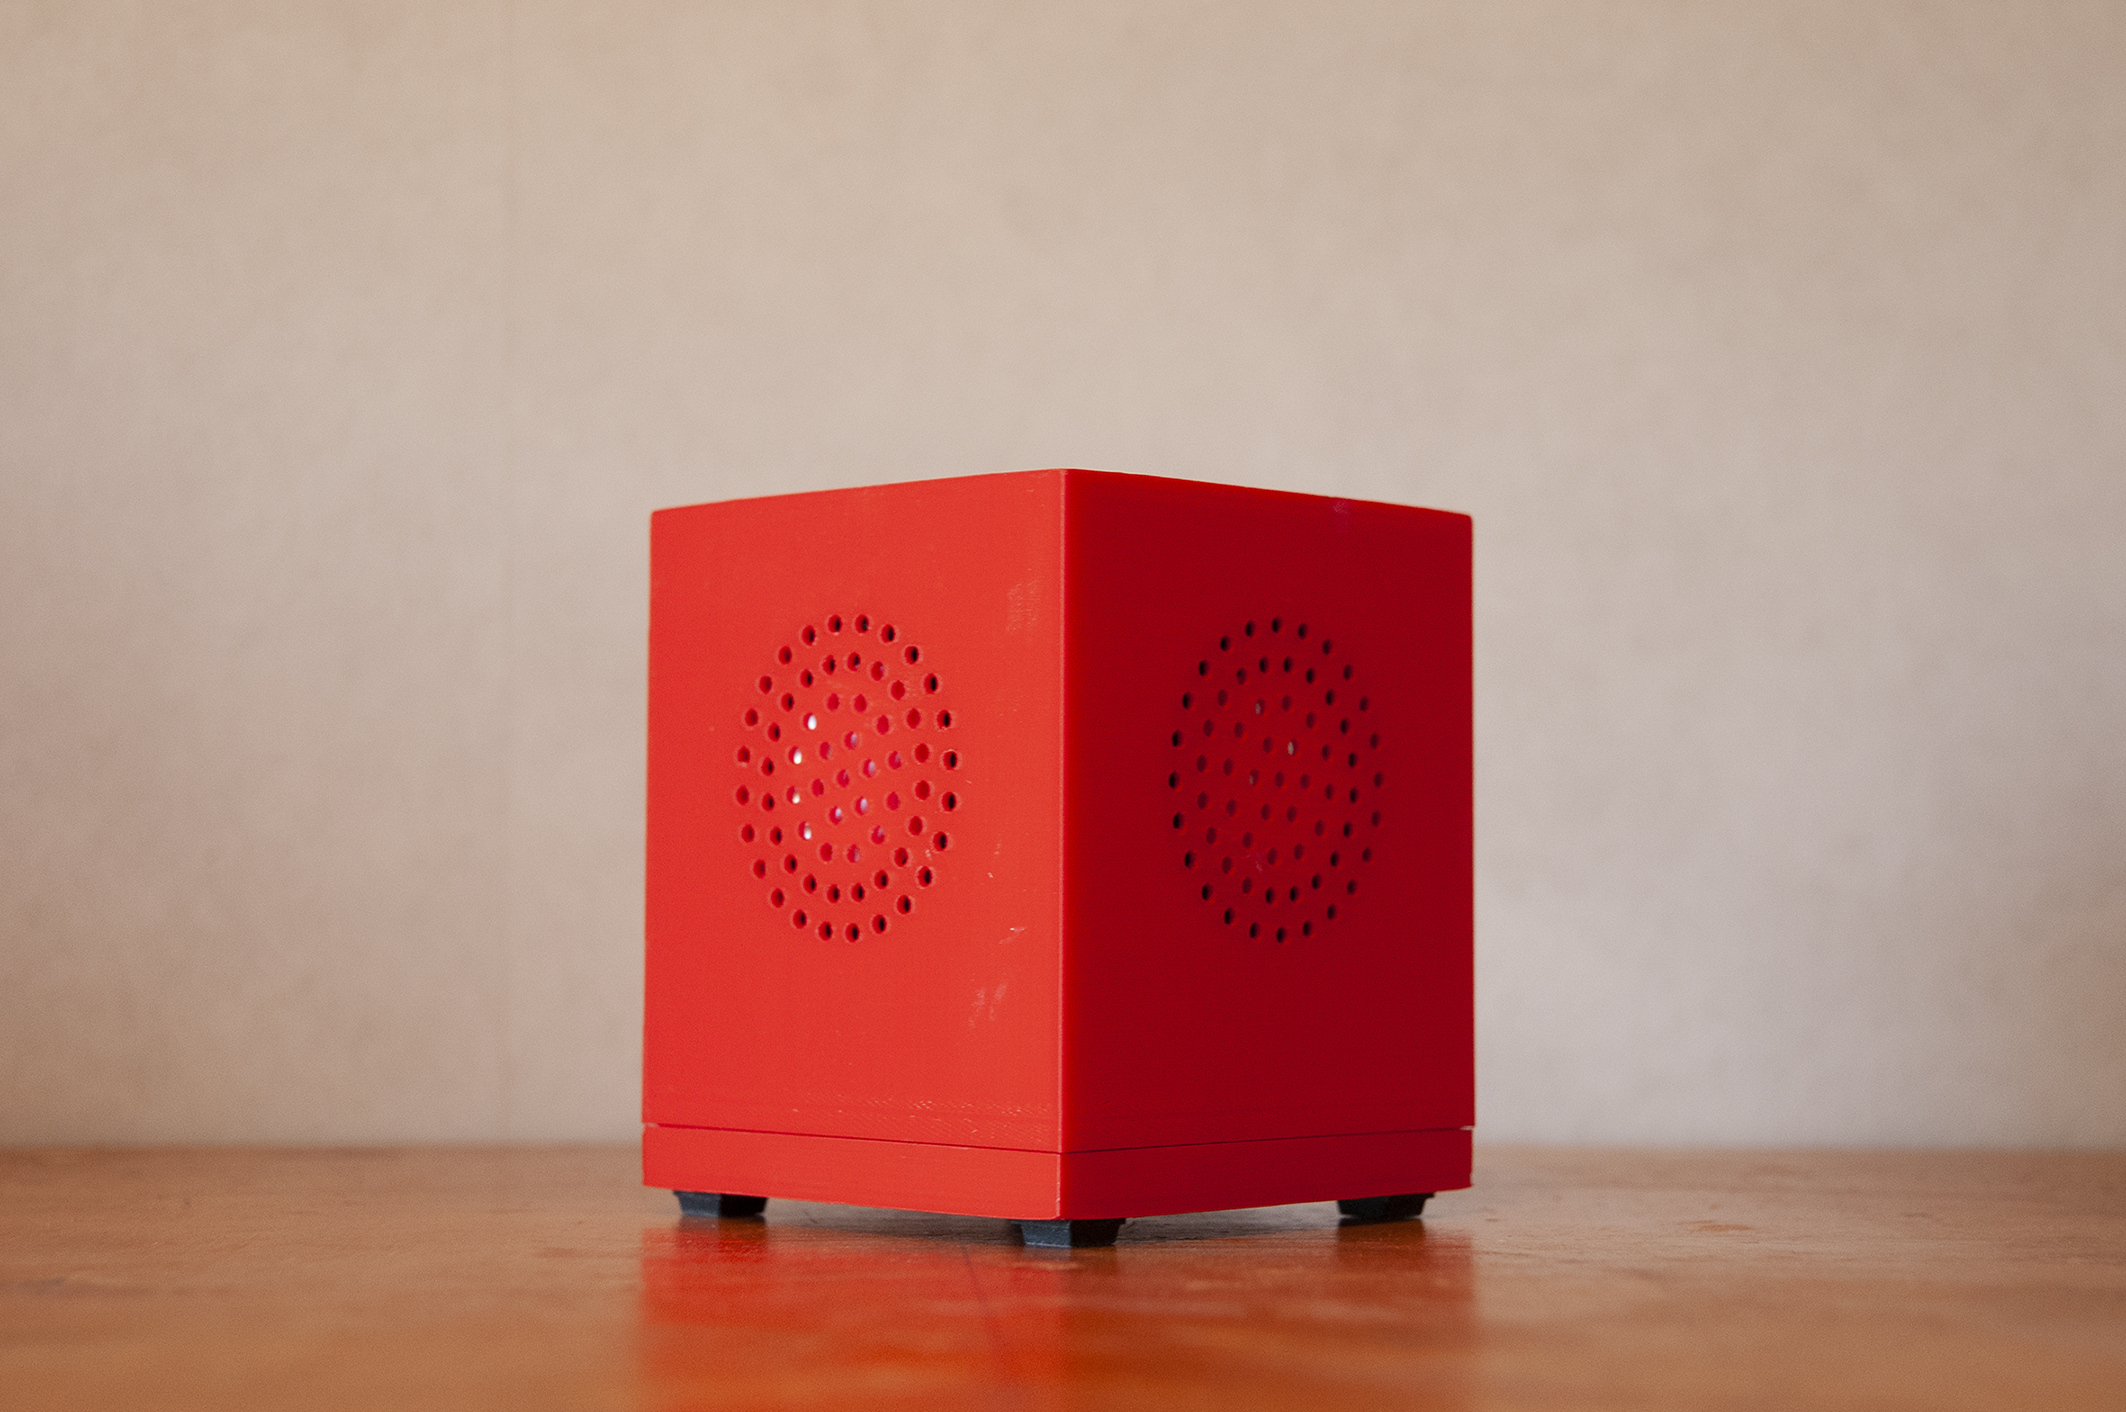
\includegraphics[width=14cm]{bilder/finale_unit_small.jpg}
    \label{fig:finale_unit} 
\end{figure}

